\chapter{根与翼} % Introduction chapter suppressed from the table of contents

中国社会一直非常强调家庭价值观，希望实现家族的持续传承，家族有族谱，代代相传的关系对每个家庭成员的成长产生深远影响。我们每个人都只是人类进化过程中的短暂过渡。父母普遍希望把最好的东西传承给下一代。然而我们需要问自己，什么东西能够持久，仅仅是财富和金钱吗？

继承大量财富，但如果不懂得如何正确利用，可能反而会削弱个人的竞争力，适得其反，最终成为社会的蛀虫。\\
《七个习惯》的作者史蒂芬•柯维（Stephen
Covey）在书的结尾（最后一章）中提到，我们可以传承给下一代并具有持久价值的，只有2样东西：根和翼。\\
``There are only two lasting bequests we can give our children - one is
roots, the other wings.''

\hypertarget{ux6839}{%
\subsection{根}\label{ux6839}}

回看人类过去130年，除了打了2次世界大战外，也做了很多前所未有的创新：

\begin{itemize}
\tightlist
\item
  电灯 （煤气灯）
\item
  汽车 （马车）
\item
  飞机
\item
  摩天大厦
\item
  半导体，集成电路
\item
  计算机
\item
  互联网
\item
  移动电话
\end{itemize}

回顾人类的创新历程，我们现在使用的许多发明，实际上都是“发明者”基于前人的经验不断演化而来的成果。我在爱丁堡大学的古乐器博物馆见到过各种奇形怪状的古乐器，它们都是现代乐队中铜管和木管乐器的前身，如双簧管、单簧管、巴松管、圆号和小号等。就像达尔文先生在《物种起源》中描述的物种进化一样，经过优胜劣汰，最终演化成现代的乐器。

例如我们熟悉的口琴和手风琴，其实是欧洲人在中国传统乐器笙的基础上改造而来的。\\
人类创新并不仅限于前述领域，这只是我们看到的凤毛麟角，在医疗、电影、音乐、数学等众多领域，同样展现出了非凡的创造力。这些都是祖先留给我们的宝贵财富。

举例来说，如果19世纪欧洲城市的居民能够坐上像“Back to the Future”那样的时间跑车，见到200年后现代人的生活，他们将感到难以置信。

正因为每一代人传承并发展了前人的成果，我们才能取得现在的成就。这，便是我们的“根”。 


\hypertarget{ux7ffc}{%
\subsection{翼}\label{ux7ffc}}

除了“根”的传承，祖先还留给了我们“翅膀”，赋予我们自由思考、打破负面基因传承的能力，而不仅仅是简单地将基因传递给下一代。\\
以下面2故事介绍2种不同的策略。 


\hypertarget{ux98deux884cux5b9eux9a8c}{%
\subsubsection{飞行实验}\label{ux98deux884cux5b9eux9a8c}}

自古以来，人类就渴望飞翔，东西方对此都曾有过诸多尝试，但大多以失败告终。传说明代火箭专家万户陶成道在凳子上绑了47根火箭，并绑上风筝进行飞行试验，最终却因爆炸丧命。15世纪，意大利的达•芬奇也曾尝试模仿鸟类翅膀设计飞行器，但也仅仅是停留在图纸上，并未实现。

\framebox{%
\begin{minipage}[t]{0.97\columnwidth}\raggedright
莱特兄弟（Wright brothers）在1903年成功进行了机动飞机的首次飞行。在12月17日的第四次飞行中，他们在空中飞行了59秒，航程达到了259米。

%\href{文件:1903wrightScreenshot_2022-02-14_103500.jpg}{300px}\\
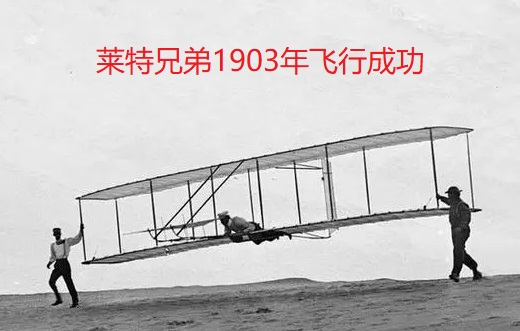
\includegraphics[width=10cm]{404页替换图片.jpg}

莱特兄弟并非工程学或数学方面的天才，但他们为了实现“飞翔”的梦想，不断从失败中吸取教训并持续改进。从1899年起，他们开始不断试验：\\
1900年，他们首次试验滑翔机，但效果并不理想。\\
1901年，他们将机翼面积从15平方米扩大到26平方米，并成功飞行了120米，但发现试验数据与计算数据不符。为了找出原因，他们制造了风洞来测量各种机翼设计的浮力，共试验了200种机翼设计。利用收集到的数据，他们开始制作第三架滑翔机。\\

到1902年9月，莱特兄弟已完成了1000次试飞，其中空中飞行时间最长达到了26秒。正因为有了这些经验，他们设计了飞机的舵，使飞行员能够更好地操控飞机，随后他们开始设计使用四缸发动机和螺旋桨的机动飞机。

1903年成功飞行后，他们继续改善设计。\\

到1905年10月，飞机已经能够在空中飞行39分钟，并能在飞行员控制下完成转圈。\\

飞行就是在不稳定的大气条件下操控一台同样不稳定的机器，充满了各种变数，因此极其困难。然而，莱特兄弟通过反复试验，发明了许多关键部件，如机翼、舵、发动机和螺旋桨等，并研究了它们之间是如何相互影响的。 

\strut
\end{minipage}}

莱特兄弟的飞行故事告诉我们，他们的成功绝非偶然。除了强烈的意念和冲劲，更为重要的是他们从自己和前人的失败中汲取经验教训并不断试验，通过数据收集和持续改进，最终实现突破。

\begin{description}
\tightlist
\item[]
= = = =
\end{description}

两年后的1905年，在大西洋对岸，瑞士伯尔尼（Bern）的一名26岁专利局员工发表了5篇科学论文，其中第4篇提出时间与空间并非固定，而是相对观察者的移动，这一观点打破了三百年以来对牛顿力学的传统认识。这篇后来被认为是物理界最具影响力的论文就是爱因斯坦的《狭义相对论》。

那么，这位年轻人是如何做到的呢？答案在于好奇心和年轻人无限的想象力。

他的好奇心源自之前物理学家在实验中发现光速是不变的，但这一发现与牛顿的传统力学相冲突。但他不是理学家，也没有实验室可供实验，只能凭借想象力，利用一系列假想的实验，创造了狭义相对论的公式。 


\framebox{%
\begin{minipage}[t]{0.97\columnwidth}\raggedright
他假设光速为C，高速火车从地板到车顶的高度为C/2，光从火车的地板射到车顶后，再反射回地板，总共耗时1个时间单位。

假设高速火车以高速v从左往右运行，一位静止的人从外面看这火车，也看到光从火车地板射到车顶，然后反射回到地板，因火车已经往右移动了vt，所以光线的总长度是Ct (\(= Ct/2 + Ct/2\))。  如果光速C是永恒不变的，那么时间t必须大于1才对，并且随着v的增大，t也越大。因此，在高速火车内部的时间比外部地面的时间要短。理解了因光速不变，时间相对必须变化的原理后，就能明白为什么会出现“太空飞行员乘坐高速火箭旅行30天后回到地球，发现地球上已经过去了几十年，亲人都已去世”的可能了。 


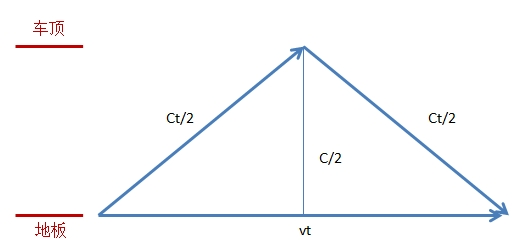
\includegraphics[width=10cm]{26章三角图.jpg}


\strut
\end{minipage}}

（爱因斯坦在后来的采访中说：“我很骄傲的是，自己有大把的空闲时间。”因为在专利局工作，所以他有很多时间，可以尽情思考、想象。)

日本数学家樱井进先生从小就崇拜爱因斯坦，他总结道：\\
“爱因斯坦教会我珍视人类所拥有的‘想象力’。想象力比知识更重要，因为知识是有限的，而想象力则概括了世界上的一切。正因为有了想象力的翅膀，人类才能抵达无法到达的地方，看到不可见的事物。我们每个人都有这样的翅膀，可以展翅高飞。”
爱因斯坦发表相对论时，大部分物理界学者认为这只是理论，无法验证，也缺乏实用价值。
科学本身就是一种喜悦，是一场旅行，旅行者能看更多其他人看不见的风景。爱因斯坦教会我们享受数学与科学研究的乐趣，而将科学应用于实际则是另一回事。 （随着科技的发展，相对论启发了后来的“宇宙大爆炸”和“黑洞”理论，并帮助我们能够精确地测量卫星的时间与定位。）


“我们都不知道。我们所了解的知识和小学生没什么两样。”爱因斯坦也曾说，“这个世界最难以理解的部分，就是去理解这个世界。”也正因为这年轻人敢面对这世界最难的挑战，使人类的物理认知上了一个台阶。他的策略是依赖年轻人无限的想象力，抛开前人留下的包袱，实现创新。


\begin{description}
\tightlist
\item[]
= = = =
\end{description}

虽然我们都继承了祖先的根与翼，但并不是每个人都能为人类的持续发展作出贡献。要具备哪些重要元素才能做到呢？ 

\framebox{%
\begin{minipage}[t]{0.97\columnwidth}\raggedright
To be a powerful transition person, one must first change his inner first. 

要成为有影响力的过渡者（a powerful transition person），无论采用哪类策略，我们必须首先进行由内而外的改变，只有这样的改变才能持久。

(只有在内部发生转变，任何人才能在自己可控的范围内进行创新和持续改善。）

以上源自Covey先生在《七个习惯》最后一章的总结。 

\strut
\end{minipage}}

\hypertarget{ux9b54ux672fux5e08ux4e54ux5e03ux65af1997ux5e74ux91cdux56deux82f9ux679c13ux5e74ux540eux518dux628aux82f9ux679cux5e26ux4e0aux9ad8ux5cf0}{%
\subsubsection{“魔术师”乔布斯1997年重回苹果，13年后再把苹果带上高峰}\label{ux9b54ux672fux5e08ux4e54ux5e03ux65af1997ux5e74ux91cdux56deux82f9ux679c13ux5e74ux540eux518dux628aux82f9ux679cux5e26ux4e0aux9ad8ux5cf0}}

1985年，乔布斯被迫离开苹果公司，独自创办NEXT公司，直到1997年NEXT被苹果收购，乔布斯重返苹果（当时苹果正处于破产边缘）。到2010年，他将苹果公司带回到美国市值最高的科技公司，这中间也经历了多次失败。

乔布斯在他的传记中说：“是什么力量推动了我？我觉得大多数创新者（Creative people）都希望感谢我们的前辈，感激他们对人类的贡献。\\

我并没有发明我用的语言或数学。我的食物基本都不是我自己做的，衣服更是一件都没做过。我所做的每一件事都有赖于前人的贡献。我们很多人都想回馈社会，在历史的长河中再添上一笔。虽然我们无法创作鲍勃•迪伦（Bob Dylan）的歌或汤姆•斯托帕德（Tom Stoppard）的戏剧，但我们可以用自己能掌握的方式去表达和体现。试图用自己的才能表达内心感受，表达对前人的感激并做出贡献，这就是推动我的力量。” 

\hypertarget{ux5171ux901aux70b9}{%
\subsection{共通点}\label{ux5171ux901aux70b9}}

为什么莱特兄弟、爱因斯坦、乔布斯能在航天、物理、电子产品领域作出突破性重大贡献？他们的故事都有两个共通点： 

\begin{itemize}
\tightlist
\item
  专注 -\/- 例如：

  \begin{itemize}
  \tightlist
  \item
    专心研究飞机
  \item
    解决物理难题，更好理解这个世界
  \item
    结合新技术研发针对个人市场的领先电子产品
  \end{itemize}
\item
  长期锲而不舍 -\/-
  从启蒙到成功都经过很多年不断努力，中间困难重重，必须内心坚定，也正是这心态让他们成为有影响力的过渡者，继续传承人类的根与翼。例如，乔布斯从被迫离开开始，前后经过25年，经过iMac iPod iPhone iPAD等，最终才使苹果再创辉煌（因为这是公司级突破，不是个人，所需时间更长）。

\end{itemize}

“你的例子都是超级明星级大人物，根与翼概念不一定适用于我们这些普通人群。”\\
“为什么你认定自己不能成为有影响力的过渡者？”我问。\\
每次听到这类反驳，我都会接着讲我的故事。 

\framebox{%
\begin{minipage}[t]{0.97\columnwidth}\raggedright
因从小很喜欢看书，从小学到大学毕业，一切都很顺利，没有遇过什么挫折。例如，因80年代香港经济仍在高速发展，大学毕业后不难找到高薪岗位，每年还有两位数的调薪，所以对自己的能力信心爆棚，也看不到自己的问题和弱点。

但香港缺乏研发工作，1992年我31岁，第一位小孩出生时，我的工程职业生涯已到了天花板。如果要继续提高收入，必须转到市场和销售岗。但转销售后，虽然能达标，但一直没有突出的表现，最终在2000年被公司辞退，沦为失业者。失业后我审视自己的问题和不足，发现自己一直以来保持着工程师思维，总觉得只要方案优良、产品有竞争力，客户就没有理由不买！但不知道产品只是商务购买中的一个考虑因素，市场如战场，有太多的因素会导致失败。最关键的是自己一直没有这种意识，也不觉得有问题。

现在静下心来想，自己一直都是先制定总体计划（最短也几个月），然后按计划执行的传统工作模式，这方式在8、90年代香港没有问题，但2000年后市场环境快速变化，思路必须转变过来，当时也刚读完软件工程，学过敏捷和精益等概念，自己的工作方式也转为每一小步试验，有效果才做下一小步的做法。例如写这本书里，每写完一个章节，必须找我的``写作伙伴''们看看，让他们给反馈，有些专门挑语法问题，有些能专门看出总体架构问题。经过他们的反馈，我再修正，然后才会在公共媒体上发布。

现在静下心来想，自己一直都是先制定总体计划（最短也几个月），然后按计划执行的传统工作模式，这方式在8、90年代香港没有问题，但2000年后市场环境快速变化，必须转变思路。当时我刚读完软件工程，学了敏捷和精益等概念，自己的工作方式也转为每一小步试验，有效果才做下一小步的做法。例如在写这本书时，每写完一个章节，必须找我的“写作伙伴”们看看，让他们给反馈，有些专门挑语法问题，有些能指出总体架构的问题。经过他们的反馈，我再修正，然后才会在公共媒体上发布。

想尝试创业，但创业很难，风险非常大。不能用传统方式，先制定大计划再执行，而是不断尝试各种能产生收入的机会，看效果。因此，开头几年我试过各种工作，比如给企业做项目管理培训，进高校当讲师，帮朋友公司做市场调研与分析，并写产品推广方案书等等，为自己带来一些收入。因因为刚读完软件工程，在富士通工作时，我也与一些CMMI5级软件开发公司合作过，就开始探索软件工程的质量改进并参与CMMI评估，慢慢学习（因毕业后一直没做过软件开发）。


从2006年开始，香港政府鼓励软件开发公司使用CMMI模型做评估与改进，并提供资助。我便开始专注于软件开发CMMI过程改进的培训与评估，并从长三角地区开始，与大陆公司合作提供CMMI服务（虽然我的成本较高，但CMMI源自美国，绝大部分材料都是英语，与大陆高校老师比较，我是直接读英文原文，比单看中文翻译能更好理解。）

十年后，2016年左右，越来越多团队使用敏捷开发，我便开始深入比较各种敏捷开发方法。2018年，正值美国PMI推出ACP个人证书，我开始与培训机构合作教授学生ACP，发现如果团队能在每次迭代回顾中利用数据（缺陷和返工）分析根因，能够更有效地提升（背后其实是改善，CMMI， 敏捷，精益等原则）。


随着接触的开发团队越来越多，我发现要有改进动力不仅仅是工程的问题，又开始探索人性相关问题（虽然以前读MBA时接触过，现在再细读X-Y理论、组织发展（Organization Development）的方法与理论）， 并在培训和现场辅导中不断实验有效的方法帮助团队提升。


学习敏捷大师和软件工程学院科学家与学者等前辈们的贡献，成为我的软件工程的根，没有他们，我不可能从零自己创造这么多东西出来。 不固步自封，因市场环境变化，从传统模式改变为精益思路，是我的翼，这这些都是我自身根和翼的经历，让我成功走过24年的独自创业之路，也帮助我成功出版第一本书（也希望这本书能为软件工程做些微小的贡献）。
根与翼如果能用得其所，确实能促进自己成为有影响力的过渡者。 

\strut
\end{minipage}} 

所以任何人，只要把心态转过来，并能锲而不舍，都有机会。”我总结说。\\
“好吧。但你说这些跟敏捷开发、持续改善有什么关系？我没有期望能成为爱因斯坦！” 

我认识的很多软件开发公司，虽然已经进行了多轮CMMI评估（每三年一轮），但一直没有任何实质的改善，是什么原因呢？

他们误以为CMMI是一套最佳过程，只要完全按照这个标准执行，开发质量便能得到保障。

美国软件工程协会在设计这个模型时，考虑到团队每个岗位都要有用，因此覆盖的范围很广，除了软件工程 从需求到最终验证确认外，还包括项目管理、配置管理、PDCA 试点与推广、度量与根因分析等。虽然模型是面面俱到，但企业在使用这个模型进行PDCA过程改进时，每一轮试点应只针对最大的痛点进行改善，显著改进后再针对次要痛点进行改善，最终满足模型所有实践范围。因此，每当美国软件工程协会（CMMI模型原创机构）听到某企业能在12个月内从零开始，迅速“高效”达到三级评估要求时，都会觉得这是不可思议的笑话。

与成为有效过渡者的要素一样，企业、团队、个人要有效改善，必须有针对性，大部分企业没有利用数据、找根因、做改进。所以开始时应只针对缺陷排除和返工工时，每次迭代回顾时分析根因。 

“听你这样说，反观我们团队，我立马想到有很多地方需要改进，例如需求调研、开发流程、持续集成、测试自动化、配置管理等。为什么你提议只针对减少缺陷引起的返工做改进？”

要理解背后的原因，先听听质量大师Dr Juran回顾过去质量改善的成功要素： 

\begin{itemize}
\tightlist
\item
  All Improvement takes place Project by Project
  所有改进只能按项目逐个进行
\item
  Backlog of Improvement projects is huge 潜在的改进项目非常多
\item
  Quality Improvement does not come Free 质量改进并非免费
\item
  Major gains come from the Vital few projects
  主要效果（收益）来自少数重要项目
\item
  Quality improvement extends to All parameters 质量改进可扩展到各类参数
  （如生产率、进度、安全性、环境等）
\end{itemize}

（以上源自 Juran 博士《 Juran Quality Handbook 》第五章质量改进。） 

所以，如果从一开始同时对4到5个方向进行改进，反而会失去聚焦，难以尽早看到改进的效果。 

但如果只针对降低缺陷引起的返工，目标明确，不仅让大家更容易接受，也更容易扩展到各个过程，例如需求、开放、产品集成，甚至配置管理。 

因为能否引起高层对改进的兴趣非常重要，所以与企业领导首次见面时，我都会讲述团队应如何分析迭代缺陷数据，以此开始定量管理。


\hypertarget{tedux6f14ux8bb2ux5f0fux603bux7ed3}{%
\subsection{TED演讲式总结}\label{tedux6f14ux8bb2ux5f0fux603bux7ed3}}

今年被质量经理邀请参加他们的质量沙龙，但只有30分钟，我就用了TED演讲思路，用了17分钟讲软件开发公司的常见质量问题和改进措施。

\framebox{%
\begin{minipage}[t]{0.97\columnwidth}\raggedright
你觉得下面4种工作，哪一类工种占的工作量最多？ 

\begin{enumerate}
\tightlist
\item
  编码与代码设计。
\item
  交付后的所有工作，包括维护、更新与缺陷修正。
\item
  交付前的评审、静态扫描、测试与缺陷修正。
\item
  项目管理与监控。
\end{enumerate}

从2012年Capers Jones对美国软件公司的统计中看到，编码只排第二（占开发工作量的25\%），而测试、评审和缺陷修改的总工作量则排第一（占30\%）。你选1.编码，其实大部分耗时的不是写代码，而是修正错误代码。软件开发有其特点，缺陷发现越晚，修复所需的工作量就越大。缺陷如果在早期被发现，可能只需要花费半小时或1小时进行修复。原因很简单，当已经集成为一个十几万行的系统，里面有很多组件。如果在完成集成后使用时才发现BUG，首先很难找到出问题的代码（原因很简单，当已经集成为一个十几万行的系统，里面有很多组件）；然后，为了验证代码修正是否有效，必须先测试单元模块是否通过，再测试集成后是否正常，最后还要通过系统测试才能交付给客户。相对而言，若能在自测、集成测试和评审阶段时尽早发现并解决问题，将节省大量时间。\\

然而，大部分缺陷都是在系统测试或集成测试时暴露的，有些产品线的缺陷数甚至达到四位数。如果能够将这些缺陷减少一半，将为公司节省近一半的工作量，同时也能改善产品质量，对吗？

道理大家都知道，但为什么没有改善？怎样才能改变现状，提前发现缺陷？

这种改进绝对不是通过下达一个命令或领导开会讲讲就能做到的。我先讲一个故事：在一家上万人的大型公司中，质量经理表示公司一直非常注重量化管理，为此制定了各种KPI考核团队，每月由主管分析数据。开始时确实有些改善，但过了一段时间后，效果就不明显了，甚至发现数据作假的情况。所以，我告诉质量经理，如果希望实现量化管理，就必须从团队提升开始，而不是仅靠总体数据分析和制定公司级改进策略。度量与分析最主要的作用在于帮助团队做好根因分析，制定纠正措施，并在下一轮迭代中进行提升。

例如，你们现在按2到4周进行一次迭代发布，确实也有一些团队在复盘，但他们不理解纠正措施与改正的区别，通常只是针对个别缺陷进行修复，结果仍会因为没有修复系统的基本问题而导致缺陷和事故重现。然而，如果整个团队在每轮迭代中分析数据、找出根因并制定纠正措施，并在下一个迭代中验证这些措施的有效性，就能养成良好的习惯。最重要的是，领导要给团队足够的时间进行复盘。要完成这种根因分析的复盘通常需要3个小时，因为要收集数据，并进行分析和讨论。

我们可以先从分析缺陷排除率入手，帮助团队养成复盘分析根因的习惯。缺陷有真实数据，让团队分析为什么需求引入的缺陷这么多？引导团队使用“五个为什么”方法找出根因。同时，团队成员需要了解当前的质量水平。通常，问需求人员自己的质量水平如何？他们会说需求评审中发现的BUG很少，就代表质量好，但这其实是一种误解。他们在评审过程中没有发现并不表示需求没有缺陷，等到客户发现时会更糟糕。

我们还可以利用一些预测模型和统计分析的方法。在迭代中，不仅要让团队制定纠正措施，还要设定定量化目标。例如需求评审应该发现多少缺陷？单元测试应该发现多少缺陷？如果未达到预期目标，说明可能还是会遗漏不少缺陷。通过设定这些目标，可以更好地推动团队进行前期的评审和单元测试。 如果团队开始养成分析根因并制定纠正措施的习惯，而领导又关注团队的持续改进，时不时地询问“下次迭代是什么时候？改进了多少？”，就可以扩大根因分析的范围。除了分析缺陷外，还可以把根因分析扩大到其他改进方向。

那么，如何开始呢？

只是把小孩扔进海里，他是学不会游泳的。因此，建议先进行培训，举办为期两天的工作坊，利用一些真实数据带领大家进行根因分析的互动练习，然后安排公司内部教练辅导团队，帮助他们在迭代中做好复盘。


\strut
\end{minipage}} 

%与企业领导的首次见面，我也会讲以上内容，说明团队如何分析迭代缺陷数据，开始定量管理。\\
%开始时如何能引起对方改进的兴趣很重要。

如果有老师或教练教授各种分析技巧，并帮助大家客观地看到团队的水平，大多数团队会对降低客户缺陷率和返工的明确量化目标产生兴趣，愿意一起分析迭代缺陷和返工量的数据，制定下一轮的改进计划与措施（好比《汤姆历险记》里，Tom认为给花园栅栏涂漆是件极富挑战，一般人难以做好的任务，他的朋友圈都会很想参加，甚至愿意付Tom礼物）。相反，如果目标仅仅是为了公司顺利通过每三年一次的评估，很多人可能会说后面的3到6个月很忙，没有时间。 


但任何显著的提升同样需要有他们内心思维的转变。 改变固有的思想和习惯并不容易。如果个人、团队或企业没有改变思维，满足于现状，觉得暂时不需要继续改善，敏捷大师提供的敏捷宣言、12条原则和各种方法（如SCRUM、XP），并进行相关的培训和技巧学习，最终都无法在敏捷开发中产生实际效果。 

反之，如果个人和企业领导对当前的工作状态都不满意，从内心深处相信必须改善质量、有危机意识，认为这些是工作的重要组成部分，是唯一能真正完善的，那么在改善过程中，或许不必单纯依赖敏捷原则和方法，甚至可以创造出更好的方法与技巧。 

团队和企业要健康成长依赖以下主要因素（与上一章创新的要素类似）：\\
*高层要制订高的目标，也要提供资源。

\begin{itemize}
\item
  \begin{itemize}
  \tightlist
  \item
    可参考开始过程改进之旅里面的获取高层支持，尽早估算改进能节省多少成本，要求立项，把过程改进作为项目来管理。
  \end{itemize}
\item
  改进要有专注。

  \begin{itemize}
  \tightlist
  \item
    例如针对如何减少缺陷返工，尽早在评审和前期测试发现缺陷，如何做好迭代回顾部分能帮助团队了解应如何开始。
  \end{itemize}
\item
  团队成员的能力与动力。

  \begin{itemize}
  \tightlist
  \item
    个人提升、自我管理、代码质量等部分能帮助提升。
  \end{itemize}
\end{itemize}

有竞争才有进步，不知道自身的不足，缺乏危机感是改善的最大阻力。 

\framebox{%
\begin{minipage}[t]{0.97\columnwidth}\raggedright


东北虎作为濒危物种，目前在国内的数量估计不超过30只，因此国家动物保护组织采取了多项措施予以保护，其中包括人工饲养。专家曾试图将这些人工饲养的东北虎重新放归野外，但这一任务极为艰巨。它们是否能够在野外独立存活下来，仍然是一个未知数。有一部纪录片生动地讲述了动物保护组织在这一过程中所面临的各种挑战和困难。

要确保老虎在野外能独立生存，它们必须能够自行觅食。在自然环境中，它们主要的捕猎对象就是鹿，但鹿非常敏捷，时速可达50公里，而且具备很强的耐力。因此，专家需要评估老虎是否能够成功捕猎到鹿，否则就不能将它们放归到野外。在评估过程中，专家发现老虎的奔跑和狩猎能力明显不如野生老虎，因为缺少运动，它们缺乏狩猎的能力。因此，专家设计了多种锻炼方法，如使用车辆牵引轮胎，并插上鲜肉块来刺激它们奔跑。经过一系列的锻炼，老虎的体力得到了恢复，但能否成功捕猎到鹿仍然是未知数。接着试验是用汽车拖着鹿的尸体吸引老虎奔跑。然而，有些老虎因为在平时的饲养过程中并没有吃过鹿肉，所以对此并不感兴趣。最终只有两三只老虎追着汽车跑，试图抓到鹿。最后有2只年轻的老虎获胜了。但要将鹿的尸体作为奖励喂给获胜的老虎也并不容易，发现它们对着鹿的尸体不知道如何下口，因为以前都是由饲养员将肉切好后喂给它们吃。最终这2只老虎花了数小时才慢慢学会如何吃到鹿肉。

\strut
\end{minipage}} 

环境是影响团队能力与动力的重要因素。看完这部纪录片，我立刻想到了有些本来很有抱负的年轻程序员，也是同样受到环境的影响。公司大部分程序员都只是天天赶工，不注重质量，管理层也习惯了大量的缺陷等到后面测试阶段才暴露，大量返工这种生产方式，如何能希望这些年轻的程序员注重代码质量。跟保护区把饲养的东北虎放归野外一样，但这些新人几个月后也习惯了大家的工作模式，后面要改变习惯便非常难。需要经过艰苦的培训，才能提高大家的竞争力。关键是管理层必须认识到，如果自己也满足于当前的模式、质量水平，对产品质量和不断改进没有要求，那么公司的产品质量将永远无法提高，也难以与其他公司竞争。

针对软件开发，我们这一代继承了之前从60年代以来的各种硬件软件的创新，给予我们继续发展的“根”。\\
敏捷宣言指出了传统瀑布式开发和传统计划驱动开发的弊端，给我们“翼”，为有能力的团队提供了机会，可以更快速地开发出高质量的产品。\\

千万不要误以为这过程会一帆风顺，按计划执行就能达到目标。实际肯定会遇到种种无法预料的问题，但只要个人、团队、企业了解当前水平，分析根因，采取纠正措施、持续改善，像第一章丰田方式的习惯4：“持续改善没有停止”—— 龟兔赛跑里的乌龟。\\

以上简单道理不仅适用于敏捷开发，但回顾周围，有多少人、团队能做到？\\
即使知道了最佳实践方法，如果没有动力（心态转变），最终只是梦想。\\
反观我的动力是什么？虽然软件工程发展历史不长（50年代才出现第一台大型计算机），但发展速度惊人。环顾周围，几乎难以找到没有附带软件的产品。 在此过程中，我们受益于软件工程的前辈，包括软件工程学院的 Humphrey先生，发表敏捷宣言的17位敏捷大师等，以及质量改善和组织发展的研究，如 Juran 博士、Lewin 教授、Weisbord 先生等。希望在我有限的能力和时间内，尽可能系统地总结这20多年与软件团队交流中的所见所闻和经验教训，解读敏捷开发最佳实践，供大家参考。 


\framebox{%
\begin{minipage}[t]{0.97\columnwidth}\raggedright


太太趁中秋长假邀请我跟她一起参加丽江香格里拉五天雨崩徒步旅行团。我们在丽江汇合后，晚上她就问我：“我的同事都说当你老公真辛苦，放假还要跟你徒步五天，没有休息。你朋友一般放假去哪里旅游？”

我没有回应，只是微笑，但心里想：“其实我认识的老朋友大部分都是选择去日本泡温泉、观光名胜、吃当地美食等，没听过参加这种徒步团。” 因为海拔高超过三千米，而且要赶早班飞机，早上四点钟就要起床，全程五天我身体都不舒服。最终还是能按行程走完。旅程结束，她回香港继续上班，我也继续飞石家庄在大陆出差。我回想今次经历：虽然身体不适，但过程中深深感受到伴侣间的理解、关怀、支持，甜在心中。旅程过后，身体慢慢恢复后，我反思： 

\begin{description}
\tightlist
\item[]
\emph{头疼、反胃、呕吐不代表心里觉得痛苦；}

\emph{快慰、舒适不一定觉得快乐。}
\end{description}

关键是如何选择面对，用心去克服困难，之后享受的喜悦更难能可贵，也帮助个人成长。

如果大家幸运，公司高层理解不断改善的重要性，给团队资源，提供培训，也希望你和我一样能正面去面对过程中的遇到的各种困难，不仅是你的宝贵经历，也帮助你成长为A级队员。个人受益，公司也受益。 



\strut
\end{minipage}} 

\hypertarget{ux53c2ux8003-references}{%
\section{参考 References}\label{ux53c2ux8003-references}}

\begin{enumerate}
\tightlist
\item
  Covey, Stephen R. \emph{The Seven Habits of Highly Effective People.}
  (1990) Fireside Book\\
\item
  Isaacson, Walter. \emph{Steve Jobs.} (2011)\\
\item
  Juran, Joseph M.   ''Juran's Quality Handbook'' (5 ed., 1999) McGraw - Hill (2011)\\
\end{enumerate}


